\documentclass[12pt]{article}%
\usepackage[T1]{fontenc}%
\usepackage[utf8]{inputenc}%
\usepackage{lmodern}%
\usepackage{textcomp}%
\usepackage{lastpage}%
\usepackage{geometry}%
\geometry{a4paper,left=20mm,right=20mm,top=20mm}%
\usepackage[english,russian]{babel}%
\usepackage{parskip}%
\usepackage{amsmath}%
\usepackage{graphicx}%
\usepackage[separate-uncertainty=true]{siunitx}%
\DeclareSIUnit\rpm{rpm}%
\usepackage{ragged2e}%
\usepackage{booktabs}%
%
\date{}%
\title{Отчет по лаботраторной работе №1.3 "Эффект Рамзауэра"}%
\usepackage{url}%
\usepackage[sorting=none]{biblatex}%
\addbibresource{wiki.bib}%
%
\begin{document}%
\normalsize%
\maketitle%
\section{Цель работы}%
\label{sec:}%
Найти размер электронной оболочки и глубину потенциальной ямы для атома ксенона.

%
\section{Теоретические сведения}%
\label{sec:}%

        Эффектом Рамзауера называется расхождение результатов наблюдений
        рассеяния электронов на атомах инертного газа с предсказаниями
        классической электромагнитной теории.

        Рассмотрим рассеяние электронов на атоме тяжелого инертного газа с точки
        зрения квантовой механики.
        Для качественного анализа можно считать,
        что при прохождении мимо атома, электрон попадает в
        потенциальную яму глубиной $U_0$, сопоставимой по длине $l$ с размером
        атома.
        Решив уравнение Шредингера, можно найти условие для максимума
        и минимума коэффициента прохождения электрона с энергией $E$ через яму,
        что соответствует максимуму и минимуму вероятности рассеяния электрона $w$:
    %
\[%
k l =  \sqrt{ \frac{2m (E_n + U_0)}{\hbar^2} } l = \pi n%
\]%
\[%
l = \frac{1}{2} \frac{h}{\sqrt{2m \left( E_1 + U_0 \right)}}%
\]%
\[%
l=\frac{1}{2} \frac{h}{\sqrt{2m \left( E_1 + U_0 \right)}}%
\]%
\[%
k l =  \sqrt{ \frac{2m (E_n + U_0)}{\hbar^2} } l = \pi n%
\]%

        Измерив энергию первого максимума прохождения $E_1$ и первого минимума
        прохождения $E_2$, можно найти $l$ и $U_0$:
    %
\[%
l=\frac{h \sqrt{5}}{\sqrt{32 m (E_2 - E_1)}}%
\]%
\[%
U_0=\frac{4}{5} E_2 - \frac{9}{5} E_1%
\]

%
\section{Экспериментальная установка}%
\label{sec:}%


\begin{figure}[h!]%
\centering%
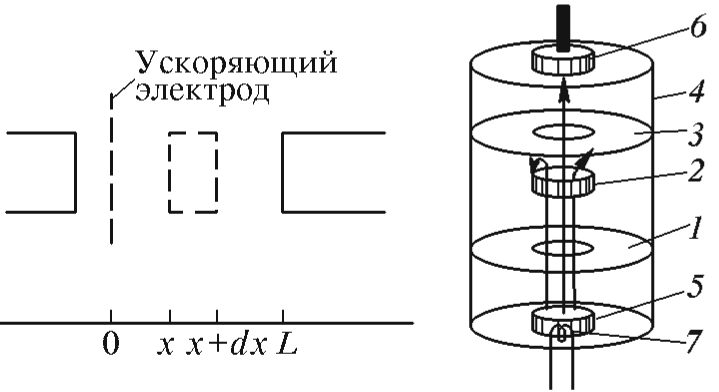
\includegraphics[width=0.8\textwidth]{sys.png}%
\caption{Тиратрон ТГ3{-}01/1.3Б}%
\end{figure}

%

        Для изучения эффекта Рамзауэра используем Тиратрон ТГ3-01/1.3Б,
        заполненный инертным газом.
        Электроны излучаются с катода $5$ и ускоряются напряжением $V$,
        приложенным между ним и ближайшей сеткой $1$. Потенциалы сеток $1$, $2$
        и анода $6$ примерно равны, поэтому поле между ними мало. Рассеявшиеся
        электроны попадают на сетки, а прошедший -- попадают на анод и образуют ток $I$.

        Посмотрим, как происходит рассеивание электронов при движении от катода к аноду.
        Пусть $n$ -- плотность газа в тиратроне, $\Delta_a$ -- поперечное сечение атома этого газа,
        $S$ -- площадь сечения тиратрона.
        Тогда в тонком слое толщиной $dx$ содержится $d\nu$ = $n S dx$ атомов газа эффективным сечением
        $\Delta = d \nu \Delta_a$. Вероятность того, что электрон наткнется на атом, равна $\frac{\Delta}{S}$.
        Тогда вероятность того, что электрон рассеется при прохождении тонкого слоя равна $W(V) = \frac{\Delta}{S} w(V)$.
        При прохождении тонкого слоя газа $N$ электронами, рассеются $dN$ электронов:
    %
\[%
dN = - W(V) N = - n \Delta_a w(V) N dx%
\]%

        Интегрируя от $0$ до длины тиратрона $L$ и заменяя число электронов $N$ на ток $I$, получаем:
    %
\[%
I(V) = I_0 e^{-C w \left( V \right)}, C = L n \Delta_a%
\]%

        Здесь $I(V)$ - ток на аноде, $I_0$ - ток на катоде.

        Измерив ВАХ тиратрона, можно найти вероятность рассеяния электронов:
    %
\[%
w = - \frac{1}{C}\ln{\frac{I(V)}{I_0}}%
\]%

        Максимальное значение коэффициента прохождения электрона равно $1$, следовательно $w(V_1) = 0$, а $I_0 = I(V_1)$.
    

%
\section{Результаты измерений}%
\label{sec:}%

        Напряжение накала $U_{\text{н}} = \qty[]{2.66}{\volt}$.
        Первоначальные измерения проводятся грубо в динамическом режиме и
        при помощи осциллографа, потом в статическом режиме цифровым мультиметром GwINSTEK GDM-8145.
    %
\subsection{Измерения в динамическом режиме}%
\label{subsec:}%
Измеренные в динамическом режиме максимум и минимум равны:%
\[%
E_1= \SI[uncertainty-mode=separate,round-mode=uncertainty,round-precision=1,separate-uncertainty-units=single]{2.8 +- 0.28284271247461906}{\electronvolt}%
\]%
\[%
E_2= \SI[uncertainty-mode=separate,round-mode=uncertainty,round-precision=1,separate-uncertainty-units=single]{7.7 +- 0.28284271247461906}{\electronvolt}%
\]%
Вычислим $l$ при известном $U_0$:%
\[%
U_0= \SI[round-mode=places,round-precision=1]{2.5}{\electronvolt}%
\]%
\[%
l= \SI[uncertainty-mode=separate,round-mode=uncertainty,round-precision=1,separate-uncertainty-units=single]{2.663626822427687 +- 0.07107428636562241}{\angstrom}%
\]%
И через $E_1$ и $E_2$:%
\[%
l= \SI[uncertainty-mode=separate,round-mode=uncertainty,round-precision=1,separate-uncertainty-units=single]{3.0971930840899606 +- 0.12641604424856984}{\angstrom}%
\]

%
\subsection{Измерения в статическом режиме}%
\label{subsec:}%

            Производитель заявляет, что точность мультиметра GDM-8145 --
            $\pm \left( 0.03\% + 4 \text{ цифры дисплея} \right)$.
            Измерение $V$ происходит в диапазоне $0-20 \unit{\volt}$,
            значит систематическую погрешность можно оценить как
        %
$\sigma_V= \SI{0.01}{\volt}$%
.
            Ток $I$ измеряется как напряжение на резисторе
            $R = \qty[]{100}{\kilo\ohm}$ в диапазоне $0-200 \unit{\milli\volt}$,
            поэтому
        %
$\sigma_I= \SI{0.1}{\milli\volt}$%
.%
\begin{center}%
\begin{tabular}{@{}S[
                table-alignment-mode = none,
                round-mode = figures,
                round-precision = 3,
            ]|S[
                table-alignment-mode = none,
                round-mode = figures,
                round-precision = 3,
            ]@{}}%
\toprule%
$V \text{, } \unit{\volt}$&$I \text{, } \unit{\milli\volt}$\\%
\midrule%
1.73&1.22\\%
1.85&4.27\\%
1.9&6.55\\%
2.09&17.1\\%
2.13&19.2\\%
2.21&21.5\\%
2.31&22.4\\%
2.41&22.0\\%
2.51&21.2\\%
2.62&20.1\\%
2.73&18.9\\%
2.8&18.1\\%
2.91&17.1\\%
3.03&16.0\\%
3.13&15.3\\%
3.24&14.7\\%
3.34&14.3\\%
3.44&13.8\\%
3.52&13.6\\%
3.62&13.1\\%
3.74&12.8\\%
3.8&12.6\\%
3.92&12.5\\%
4.03&12.2\\%
4.12&12.1\\%
4.3&11.8\\%
4.61&11.4\\%
4.94&11.0\\%
5.23&10.7\\%
5.51&10.5\\%
5.82&10.3\\%
6.11&10.2\\%
6.41&10.0\\%
6.52&9.95\\%
6.65&9.92\\%
6.84&9.72\\%
7.01&9.7\\%
7.12&9.75\\%
7.22&9.67\\%
7.32&9.7\\%
7.44&9.73\\%
7.54&9.77\\%
7.84&9.9\\%
8.13&10.1\\\bottomrule%
%
\end{tabular}%
\end{center}%


\begin{figure}[htbp]%
\centering%
\includegraphics[width=0.8\textwidth]{/tmp/pylatex-tmp.b11oof15/8ebe914c-f119-4361-8e32-42305d1c0d2d.pdf}%
\caption{ВАХ тиратрона}%
\end{figure}

%
Найдем максимум, минимум, и ток на аноде по параболической аппроксимации:%
\[%
E_1= \SI[uncertainty-mode=separate,round-mode=uncertainty,round-precision=1,separate-uncertainty-units=single]{2.3561598912360555 +- 0.011495058671964434}{\electronvolt}%
\]%
\[%
E_2= \SI[uncertainty-mode=separate,round-mode=uncertainty,round-precision=1,separate-uncertainty-units=single]{7.228885001006747 +- 0.023319467204762644}{\electronvolt}%
\]%
\[%
I_0 \approx \SI[round-mode=figures,round-precision=3]{22.490519846065638}{\milli\volt}%
\]%
Для максимума и минимума учтем систематическую погрешность:%
\[%
E_1= \SI[uncertainty-mode=separate,round-mode=uncertainty,round-precision=1,separate-uncertainty-units=single]{2.3561598912360555 +- 0.011495058671964434}{\electronvolt}%
\]%
\[%
E_2= \SI[uncertainty-mode=separate,round-mode=uncertainty,round-precision=1,separate-uncertainty-units=single]{7.228885001006747 +- 0.023319467204762644}{\electronvolt}%
\]%
Теперь рассчитаем размер электронной оболочки атома $l$ и глубину потенциальной ямы $U_0$:%
\[%
l=\frac{h \sqrt{5}}{\sqrt{32 m (E_2 - E_1)}}= \SI[uncertainty-mode=separate,round-mode=uncertainty,round-precision=1,separate-uncertainty-units=single]{3.105849197142824 +- 0.008285726227780319}{\angstrom}%
\]%
\[%
U_0=\frac{4}{5} E_2 - \frac{9}{5} E_1= \SI[uncertainty-mode=separate,round-mode=uncertainty,round-precision=1,separate-uncertainty-units=single]{1.5420201965804976 +- 0.027859509755233165}{\electronvolt}%
\]%
Оценим, где будут находится следующие 2 максимума:%
\[%
\sqrt{ \frac{2m (E_n + U_0)}{\hbar^2} } l = \pi n%
\]%
\[%
E_n = \frac{n^2 h^2}{8m l^2} - U_0%
\]%
\[%
E_{n|n=2}= \SI[uncertainty-mode=separate,round-mode=uncertainty,round-precision=1,separate-uncertainty-units=single]{14.050700154685705 +- 0.087736626739131}{\electronvolt}%
\]%
\[%
E_{n|n=3}= \SI[uncertainty-mode=separate,round-mode=uncertainty,round-precision=1,separate-uncertainty-units=single]{33.54160059376846 +- 0.18925265370486946}{\electronvolt}%
\]%
Построим график вероятности рассеяния электрона:%


\begin{figure}[htbp]%
\centering%
\includegraphics[width=0.8\textwidth]{/tmp/pylatex-tmp.b11oof15/94caa048-0f26-47c8-8991-1f9d0d21aa89.pdf}%
\caption{Вероятность рассеяния электрона}%
\end{figure}

%
\subsection{Анализ результатов}%
\label{subsec:}%
\begin{center}%
\begin{tabular}{@{}c|c@{}}%
\toprule%
&$l \text{, } \unit{\angstrom}$\\%
\midrule%
Удвоенный ковалентный радиус (\cite{enwiki:1114639486})&\SI[uncertainty-mode=separate,round-mode=uncertainty,round-precision=1,separate-uncertainty-units=single]{2.8 +- 0.18}{\angstrom}\\%
Динамический режим при известном $U_0$&\SI[uncertainty-mode=separate,round-mode=uncertainty,round-precision=1,separate-uncertainty-units=single]{2.663626822427687 +- 0.07107428636562241}{\angstrom}\\%
Динамический режим&\SI[uncertainty-mode=separate,round-mode=uncertainty,round-precision=1,separate-uncertainty-units=single]{3.0971930840899606 +- 0.12641604424856984}{\angstrom}\\%
Статический режим&\SI[uncertainty-mode=separate,round-mode=uncertainty,round-precision=1,separate-uncertainty-units=single]{3.105849197142824 +- 0.008285726227780319}{\angstrom}\\\bottomrule%
%
\end{tabular}%
\end{center}%

            Все полученные результаты сопоставимы с размером электронной
            оболочки атома, если считать его равным удвоенному ковалентному радиусу.
        

%
\section{Заключение}%
\label{sec:}%

        В ходе работы удалось пронаблюдать поведение электронов, которое предсказывалось квантовомеханической теорией.
        Получилось оценить примерный размер атома ксенона и глубину его потенциальной ямы.
    

%
\printbibliography%
\end{document}